\documentclass{article}
\usepackage[utf8]{inputenc}
\usepackage{amsmath}
\usepackage{natbib}
\usepackage{graphicx}
\usepackage{astrojournals}
\bibliographystyle{apj}
\usepackage[spanish, es-minimal, english]{babel}
\usepackage[vmargin=0.8in, hmargin=1.00in]{geometry}
%\usepackage[demo]{graphicx}
%\usepackage{floatrow}
%\caption{caption text}
\usepackage{sidecap}
\usepackage{cleveref}
\crefname{section}{§}{§§}
\Crefname{section}{§}{§§}


\setlength{\fboxsep}{0pt}%
\newlength\figwidth
\setlength\figwidth{0.48\textwidth}
\setlength\tabcolsep{0pt}
\usepackage{hyperref}
\newcommand\raiselabel[1]{\raisebox{0.39\figwidth}[-0.39\figwidth]{#1}}
%\renewcommand{\baselinestretch}{1.3}
\newcommand{\gt}{>}
\newcommand\U[1]{\ensuremath{\mathrm{#1}}}
\newcommand\msol{M_\odot}
\newcommand\msolagno{M_\odot\,\U{yr^{-1}}}

%\newcommand\U[1]{\ensuremath{\mathrm{#1}}}
\newcommand\K{\U{K}}
\newcommand\cm{\U{cm}}
\newcommand\AU{\U{AU}}
\newcommand\g{\U{g}}

\newcommand\acre{\ensuremath{_{\mathrm{acre}}}}
\newcommand\eff{\ensuremath{_{\mathrm{eff}}}}
\newcommand\Ext{\ensuremath{_{\mathrm{Ext}}}}
\newcommand\Int{\ensuremath{_{\mathrm{Int}}}}

\newcommand\ha{\ensuremath{\mathrm{H\alpha}}}
\newcommand\oiii{\ensuremath{\mathrm{[O\,III]}}}
\newcommand\A{\ensuremath{\text{\AA{}}}}

%% Commands for the postage stamp images
\setlength{\fboxsep}{0pt}%
%\newlength\figwidth
\setlength\figwidth{0.46\textwidth}
\newlength\figstampcolsep
\setlength\figstampcolsep{5pt}
\newcommand\BowshockFig[1]{
  \includegraphics[width=\figwidth, clip, trim=10 10 10 10]
  {#1}
}
\newcommand\BowshockFigImg[1]{
  \includegraphics[width=0.5\figwidth, clip, trim=350 50 350 50]                 %Images
  {#1}
}

\newcommand\BowshockFigImag[1]{
  \includegraphics[width=0.9\figwidth, clip, trim=20 20 10 10]                 %Images
  {#1}
}
%\newcommand\raiselabel[1]{\raisebox{0.9\figwidth}[-0.5\figwidth]{#1}}


\title{Discovery of a new high  ionization planetary nebula in LAMOST}

\author{Luis A. Gutiérrez Soto     
}

\begin{document}
\maketitle

\section{Introduction}
\label{sec:intro}

Planetary nebulae (PNe) represent the last stage of evolution of low- and intermediate-mass stars (0.8$\msol$ - 8.0$\msol$). The PNe phase begin when gas is ejected from the red giant stars late in their lives and subsequently this gas is ionized by the radiation field coming from the remnant star resulted. An emission nebula expands, a glowing shell of ionized gas until lost in the interstellar medium. Then the dying star core becomes a white dwarf.

The number of the PNe discovered in the galaxy is relatively low (\(\sim 3,500\)). However, this current number of PNe represents only about 15-30\% of the estimated
total of Galactic PNe (Frew, 2008; Jacoby et al., 2010) showing that a small fraction
of the PNe have been cataloged (Frew, 2017). This mean that the search for planetary nebulae becoming a important task, that eavery time is more dificult, due to many of the undiscovered PNe are probably
the more distant and then the more the weak. And because many of them, probably, are located in nuvens of dust. And note that planetary nebulae only last for about 5,000-
25,000 yr (Badenes et al. 2015), making them a very short-lived part of the stellar life cycle.
But is import to discovery new planetary nebula? the answer could be very obvious and is related with the idea that PNe provide vital clues for the understanding late-stage stellar evolution and Galactic chemical enrichment. Their strong emission lines allow the determina-
tion of abundances, expansion and radial velocities, and
CSPN temperatures. PNe yield information on the nuclear
burning, dredge up, and mass loss in the stellar progenitor
(see Kwitter & Henry 2022 for an excellent recent PN
review).

PN studies have been hampered by three problems:
(i) the previous lack of accurate distances to most Galactic
PNe; (ii) obtaining representative PNe samples of the true
population diversity (Parker 2022), and (iii) their unknown
progenitor masses. The first problem has prospects of
resolution via accurate Gaia CSPN distances, though many
CSPNe remain too distant and faint for Gaia DR3 and correct
CSPN identification remains an issue for some (Parker et al.
2022). The second problem is being addressed by deep, narrow-band, wide-field surveys, e.g., Parker et al. (2005),
Drew et al. (2005), and Drew et al. (2014). For the third problem of progenitor masses, these can only
be accurately determined for PNe in Galactic globular and
open clusters (OCs). These allow precise distance determina-
tions from color–magnitude diagrams (CMD) and Gaia.

\section{Surveys}
\label{sec:surveys}

\subsection{GAIA EDR3}
\label{sec:gaia}

\subsection{Pan-STARRS DR1}
\label{sec:gaia}

\subsection{LAMOST DR7}
\label{sec:gaia}

\section{Methodology}
\label{sec:surveys}

At the beginning the idea was to identify for new planetary nebula in GAIA. I started to constructed possibles color-color diagrams to separate PNe from other emission lines objects and stars using GAIA only. The separation was not good because PNe and other emission line stars like CVs occupy the same region in the diagram. Then, I decided to move to Pan-STARRS and combining the two surveys Pan-STARRS and GAIA. I found one color diagram that isolate the PNe with, I suppose, strong \ha{} emission line. By using the \((G - r)\) versus \((G_{BP} - G_{RP})\) color-color

\begin{figure}
\centering
  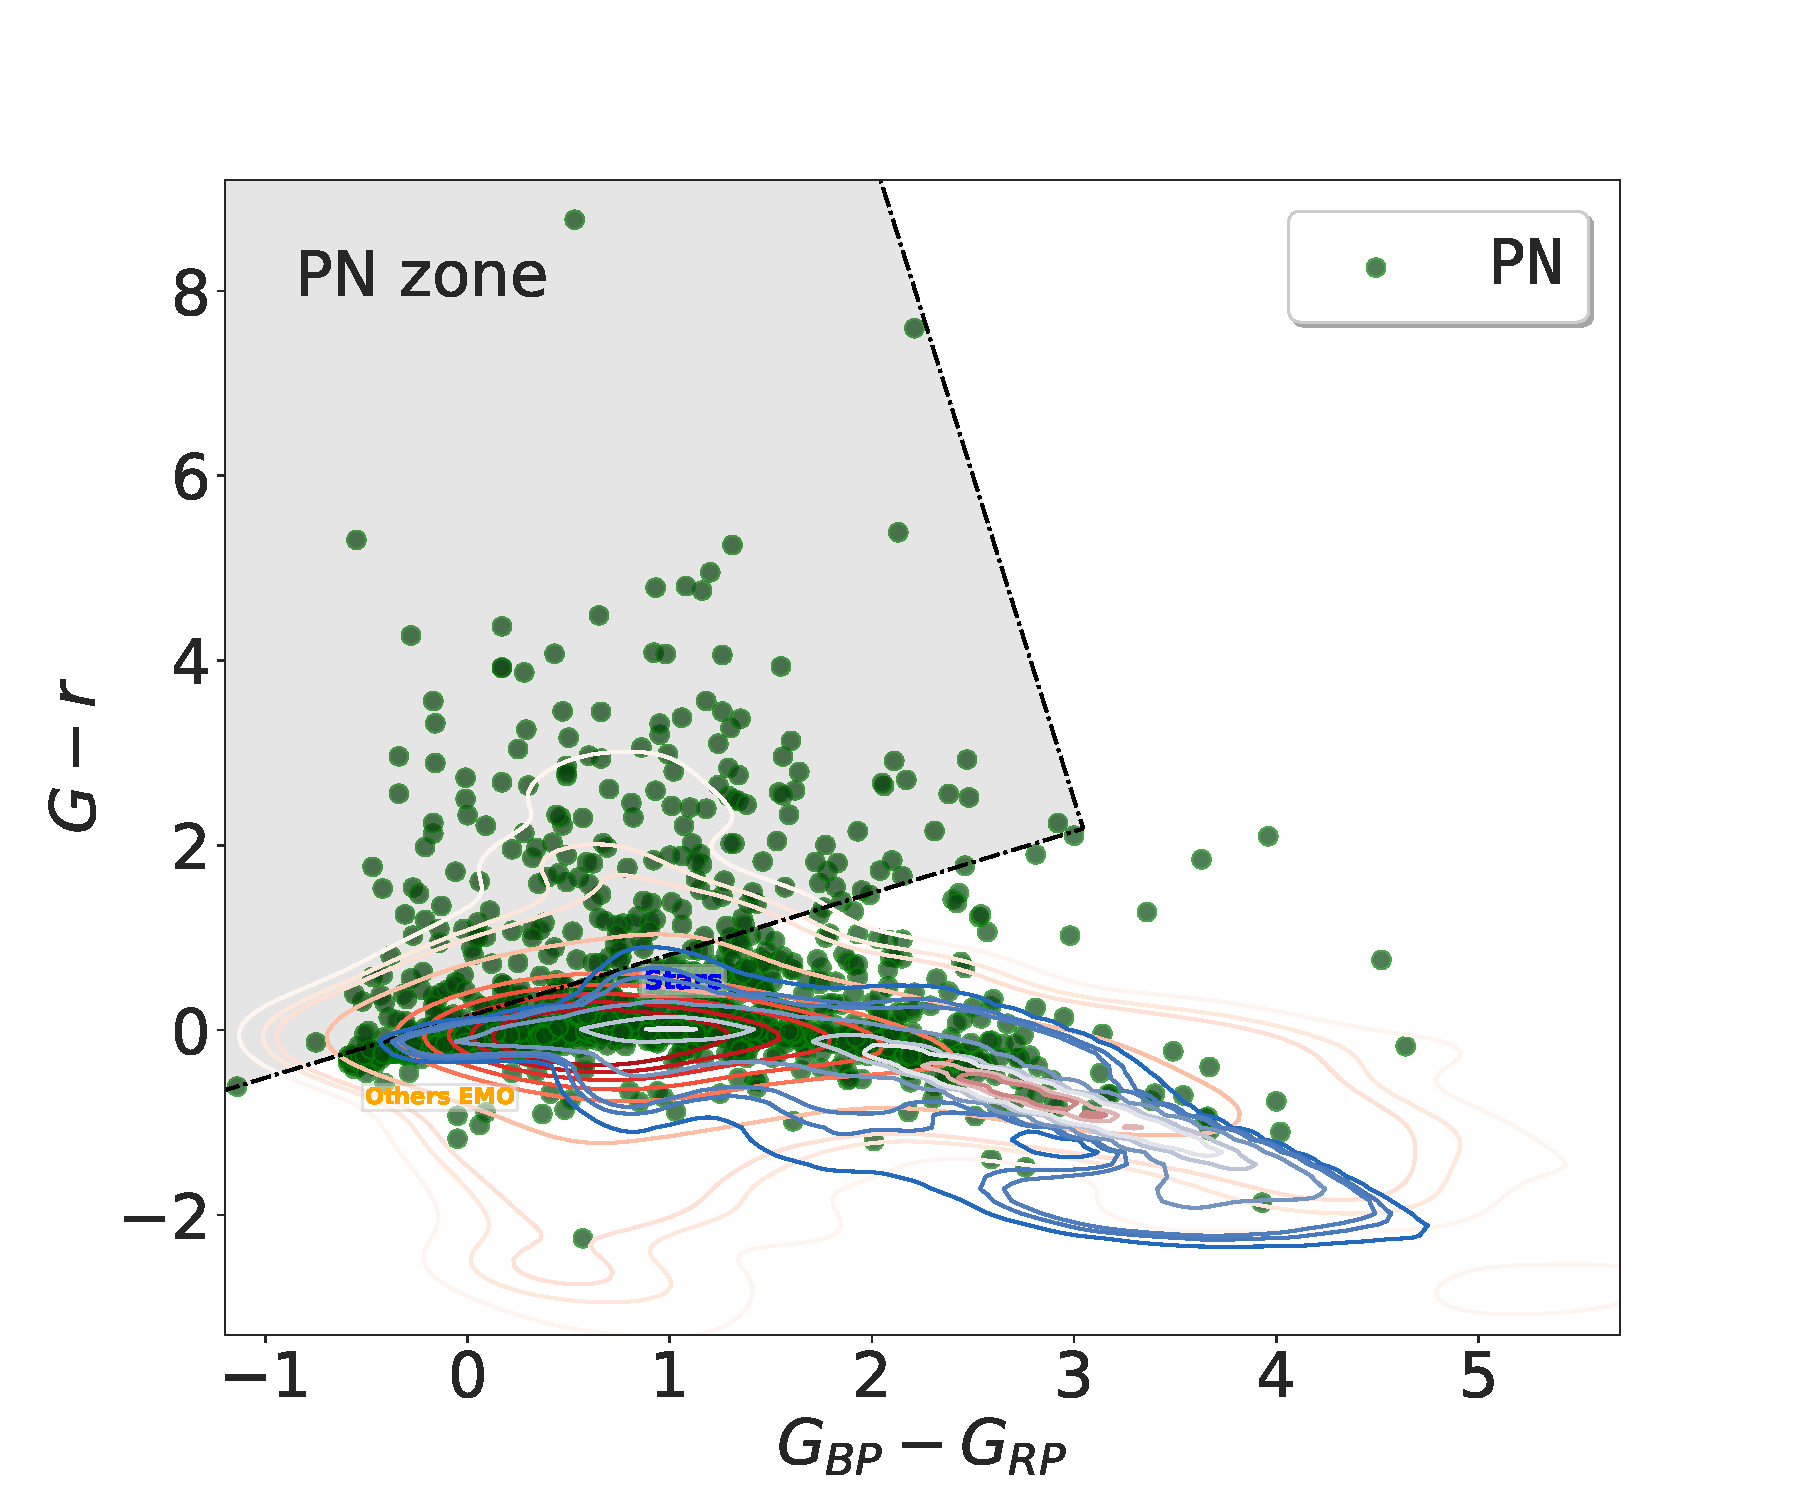
\includegraphics[width=0.9\linewidth]{../Figs/color-diagram-ps-gaiaEDR3.pdf}
  \caption{} 
  \label{fig:Viironen}
\end{figure}

\bibliography{Ref-pne}

\end{document}

